\chapter{Performance Analysis}
\label{cha:pa}

The purpose of this chapter is to examine and discuss \textit{STEERED}'s performance
impact on the code. Firstly, we present the difference in execution time between
a standard binary and a \textit{STEERED}-secured one. In this part we will give great
importance to the time overhead, describing the reason behind the collected
values. Secondly, we present the difference in size between the produced
binaries, giving great importance to memory overhead. Lastly, we provide an analysis
of the obtained results as well as some optimization ideas to further reduce the
performance impact of \textit{STEERED} on the code.

The performance analysis took inspiration from the articles \textit{Efficient
CFI Enforcement for Embedded Systems Using ARM TrustZone-M}\cite{article1} (Gisu
Yeo, Yeryeong Kim et al., 2022) and \textit{PROLEPSIS: Binary Analysis and Instrumentation
of IoT Software for Control-Flow Integrity}\cite{article2} (Valentina Forte, Nicol\`{o}
Maunero et al., 2021) where the writers propose a solution similar to \textit{STEERED}
for \textit{ARM}-based embedded devices. We tested the infrastructure on the same
algorithms proposed by the papers, providing tests on $13$ different algorithms
+ $4$ variations with indirect jumps.

Moreover, to present correct and realistic data, all tests have been conducted
on the aforementioned \textit{Espressif's ESP32-C3-DevKitM-1}.

\section{Time Performances}
\label{sec:pa_time}

In this section, we will see how \textit{STEERED}'s infrastructure affects the
execution time of the code. Two histograms depicting test results can be seen in
Figures \ref{fig:lowtime} and \ref{fig:hightime}, note that execution times have
been separated into two different charts to enhance readability.

\begin{figure}[htbp]
  \centering
  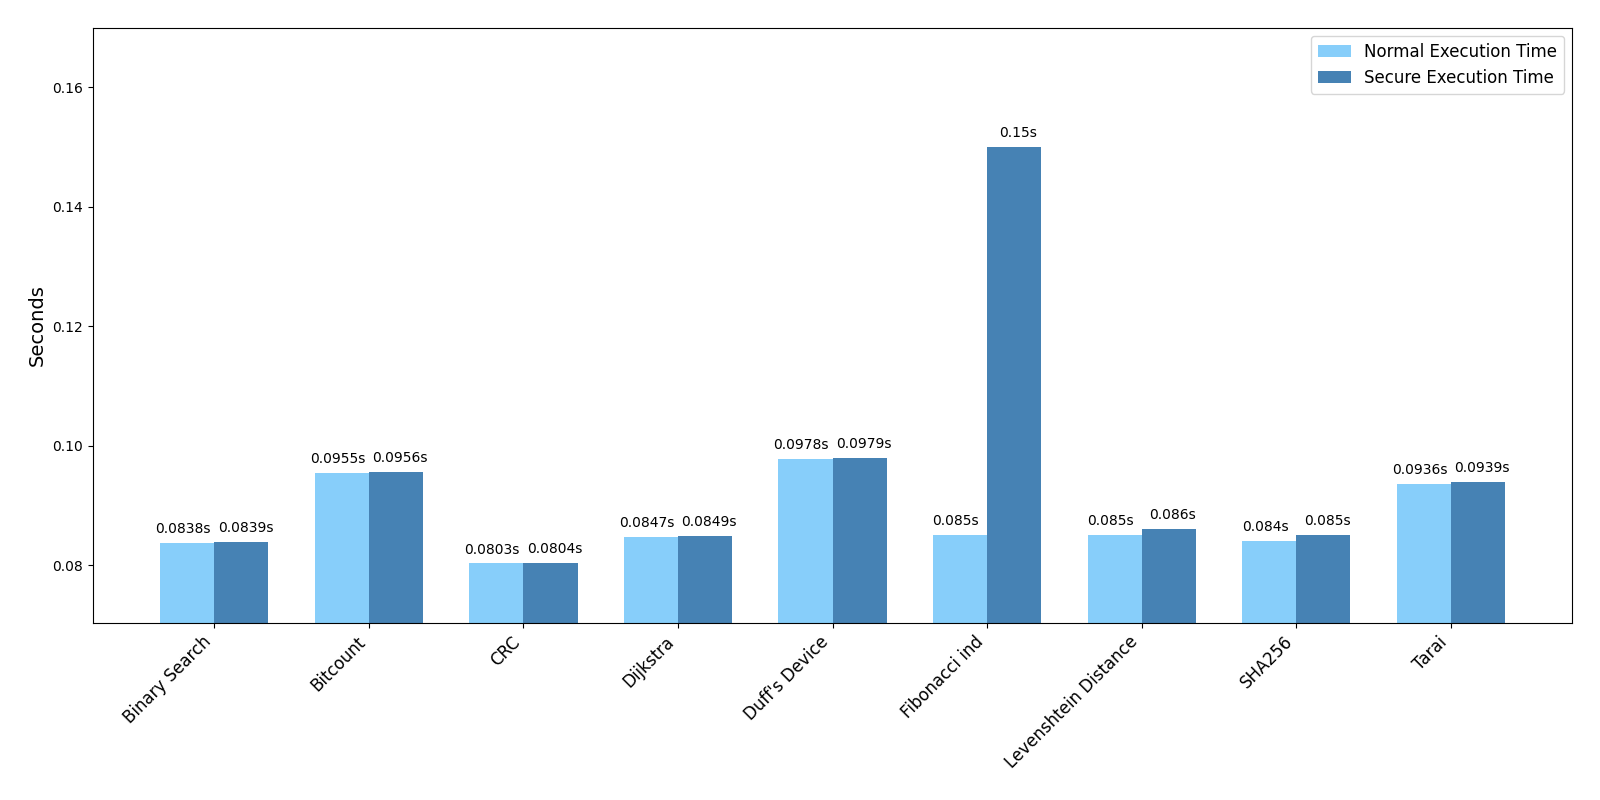
\includegraphics[width=\linewidth]{images/low_times.png}
  \caption{Comparison between binaries execution times (low times)}
  \label{fig:lowtime}
\end{figure}

\begin{figure}[htbp]
  \centering
  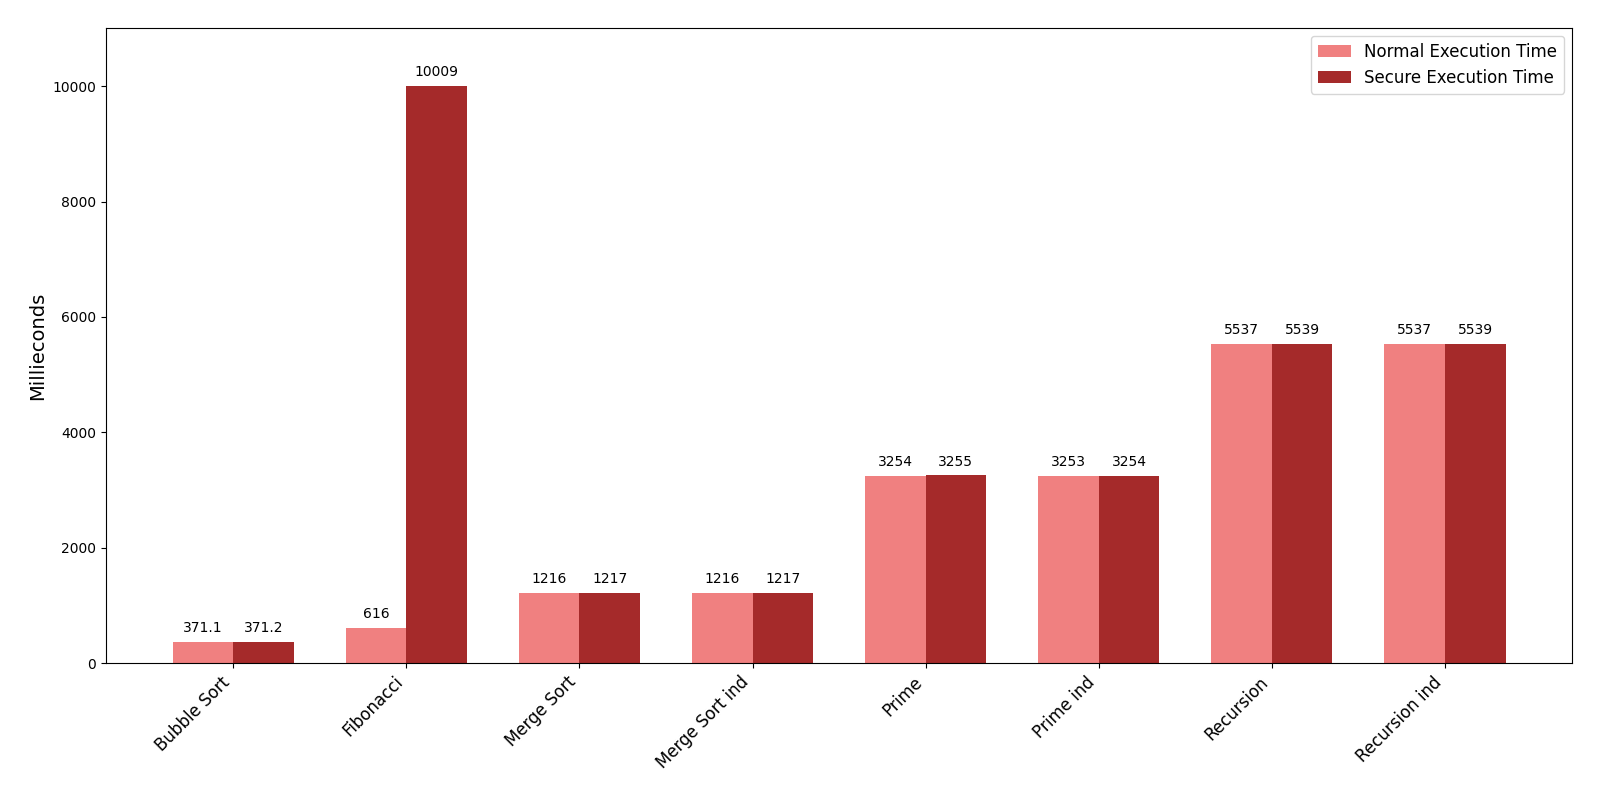
\includegraphics[width=\linewidth]{images/high_times.png}
  \caption{Comparison between binaries execution times (medium and high times)}
  \label{fig:hightime}
\end{figure}

Table \ref{tab:times} depicts test results for each algorithm as well as the
percentage of time overhead. As we can see, in most cases the time overhead
affects the fourth or fifth digit resulting in an unnoticeable increase in
execution time. However, there are two cases in which the time overhead is very
big and it impacts performances in a relevant way.

\begin{table}
  \centering
  \begin{tabular}{|c|c|c|c|}
    \hline
    \textbf{Algorithm}                   & \textbf{Normal run time (s)} & \textbf{Secure run time (s)} & \textbf{Time Overhead} \\
    \hhline{====} \textit{Binary Search} & 0.08387                      & 0.08388                      & $0.012\%$              \\
    \hline
    \textit{Bitcount}                    & 0.0955                       & 0.0956                       & $0.11\%$               \\
    \hline
    \textit{Bubble Sort}                 & 0.37113                      & 0.37116                      & $0.008\%$              \\
    \hline
    \textit{CRC}                         & 0.08025                      & 0.08026                      & $0.012\%$              \\
    \hline
    \textit{Dijkstra}                    & 0.0847                       & 0.0849                       & $0.236\%$              \\
    \hline
    \textit{Duff's Device}               & 0.097795                     & 0.097799                     & $0.0041\%$             \\
    \hline
    \textit{Fibonacci}                   & 0.6166                       & 10.0089                      & $1523.24\%$            \\
    \hline
    \textit{Fibonacci Indirect}          & 0.0849                       & 0.1511                       & $77.97\%$              \\
    \hline
    \textit{Levenshtein Distance}        & 0.085                        & 0.086                        & $1.176\%$              \\
    \hline
    \textit{Merge Sort}                  & 1.216                        & 1.217                        & $0.0822\%$             \\
    \hline
    \textit{Merge Sort Indirect}         & 1.2168                       & 1.2169                       & $0.0082\%$             \\
    \hline
    \textit{Prime}                       & 3.254                        & 3.255                        & $0.03\%$               \\
    \hline
    \textit{Prime Indirect}              & 3.253                        & 3.254                        & $0.03\%$               \\
    \hline
    \textit{Recursion}                   & 5.537                        & 5.539                        & $0.036\%$              \\
    \hline
    \textit{Recursion Indirect}          & 5.537                        & 5.539                        & $0.036\%$              \\
    \hline
    \textit{SHA256}                      & 0.084                        & 0.085                        & $1.19\%$               \\
    \hline
    \textit{Tarai}                       & 0.0936                       & 0.0939                       & $0.32\%$               \\
    \hline
  \end{tabular}
  \caption{Test results for execution times}
  \label{tab:times}
\end{table}

It is straightforward to understand why the overhead is small for algorithms like
\textit{Binary Search} and \textit{Duff's Device} since these programs perform few
jumps and most of the computation is performed inside a while or for loop so,
the overhead given by the instrumentation is unnoticeable if compared to the
total execution time. For example, the \textit{Binary Search} algorithm performs
$3$ jump instruction and $3$ return instructions even if it is working on a rather
big array. Given this behavior, such a small time overhead is expected in similar
situations.

Instead, examples like \textit{Prime} and \textit{Recursive} are a bit trickier.
Since these algorithms work with a recursive approach they perform many control transfer
instructions consequently thus, we expect the time required for the context
switch and the forward and backward edge controls to be somewhat impactful. However,
results show that even in these cases the difference is barely noticeable\footnote{In
these cases instead of impacting the fourth or fifth digit the overhead impacts
the second or third digit.}. The reason could be due to the processor's
frequency which, in the case of \textit{Espressif's ESP32-C3-DevKitM-1}, is $160
\ MHz$. This means that the CPU is able to execute the secure and non-secure
binaries in a similar time. For example, the \textit{Recursion} algorithm performs
$\sim 4000$ jump instructions and $\sim 4000$ return instructions which translates
to $\sim 8000$ edge controls and $\sim 16000$ context switches\footnote{The
number is doubled because for each edge control we need to increase the
privilege to M-mode, perform the control, and then return to U-mode, resulting in
two context switches.}. However, if we compare those numbers to the $160$
million operations the processor can perform in a second we see why the time
overhead is so small. Note that we add $2$ instructions for every jump instruction
and $3$ instructions for every return instructions, resulting in an instruction
overhead of $4000*2 + 4000*3 = 20000$. Moreover, the handling of forward and
backward edge controls requires $\sim 800$ instructions which results in
$(4000 + 4000) * 800 = 6400000$ total instructions. Now, if we compute
$\frac{20000 + 6400000}{160000000}$ we discover that the utilized processor is
able to perform all these instructions in $\sim 0.04$ seconds. Depending on the algorithm
and the recursion depth we see that the overhead is affecting the second or third
digit.

Two peculiar cases are the ones of the \textit{Fibonacci} and \textit{Fibonacci
Indirect} algorithms, in these cases, the overheads are $1523.24\%$ and $77.97\%$
respectively. The possible reason for these enormous overheads is that these
algorithms make two recursive calls each time so we end up with an exponential
amount of jump and return instructions. This leads to many edge controls and the
execution is strongly affected by this.

Overall, \textit{STEERED} achieved an average time overhead of $94.38\%$ with a standard
deviation of $368.68$. However, if we do not take into account the outliers we can
see that the median is $0.036\%$. These results clearly show that \textit{STEERED}'s
time overhead is almost unnoticeable in many cases but, this also demonstrates
that the project strongly suffers from deeply recursive algorithms and that
further optimization is required to reduce time impact on these type of
algorithms.

Lastly, in Table \ref{tab:othertimes} we provide the times required to instrument
the code, extract the CFG, and perform the simulation. As we can see the
instrumentation and CFG extraction phases always require less than a fraction of
a second to finish. However, we must take into consideration that the tested
algorithms are composed of few lines of code and the situation could change if
we were to instrument a firmware composed of thousands of lines. The simulation instead
requires a lot of time, even algorithms that run in a second or less require a
few seconds to simulate. This is due to the logging required to extract the indirect
jump destinations which affects the time performances seriously. Note that we
can accept this result since the simulation is run only once and the logging is
removed from the final binary so that this overhead is not affecting the actual
execution.

\begin{table}
  \centering
  \begin{tabular}{|c|c|c|c|}
    \hline
    \textbf{Algorithm}                   & \textbf{Instrumentation (s)} & \textbf{Simulation (s)} & \textbf{CFG extraction (s)} \\
    \hhline{====} \textit{Binary Search} & 0.00296                      & no ind jumps            & 0.00174                     \\
    \hline
    \textit{Bitcount}                    & 0.00196                      & no ind jumps            & 0.00153                     \\
    \hline
    \textit{Bubble Sort}                 & 0.00302                      & no ind jumps            & 0.00175                     \\
    \hline
    \textit{CRC}                         & 0.00203                      & no ind jumps            & 0.00154                     \\
    \hline
    \textit{Dijkstra}                    & 0.00264                      & no ind jumps            & 0.00182                     \\
    \hline
    \textit{Duff's Device}               & 0.00265                      & no ind jumps            & 0.00163                     \\
    \hline
    \textit{Fibonacci}                   & 0.00209                      & no ind jumps            & 0.00149                     \\
    \hline
    \textit{Fibonacci Indirect}          & 0.00202                      & 130.5567                & 0.07037                     \\
    \hline
    \textit{Levenshtein Distance}        & 0.00255                      & no ind jumps            & 0.00167                     \\
    \hline
    \textit{Merge Sort}                  & 0.00354                      & no ind jumps            & 0.00178                     \\
    \hline
    \textit{Merge Sort Indirect}         & 0.0036                       & 4.6394                  & 0.00273                     \\
    \hline
    \textit{Prime}                       & 0.00214                      & no ind jumps            & 0.00168                     \\
    \hline
    \textit{Prime Indirect}              & 0.00208                      & 11.4051                 & 0.00451                     \\
    \hline
    \textit{Recursion}                   & 0.00202                      & no ind jumps            & 0.00159                     \\
    \hline
    \textit{Recursion Indirect}          & 0.00202                      & 23.2751                 & 0.00875                     \\
    \hline
    \textit{SHA256}                      & 0.00411                      & no ind jumps            & 0.00189                     \\
    \hline
    \textit{Tarai}                       & 0.00198                      & no ind jumps            & 0.00152                     \\
    \hline
  \end{tabular}
  \caption{Test result for instrumentation phases}
  \label{tab:othertimes}
\end{table}

\section{Memory Overhead}
\label{sec:pa_memory}

In this section, we will see how \textit{project name} affects the size of the
produced binary (a histogram depicting test results can be seen in Figure \ref{fig:binsize}).

\begin{figure}[htbp]
  \centering
  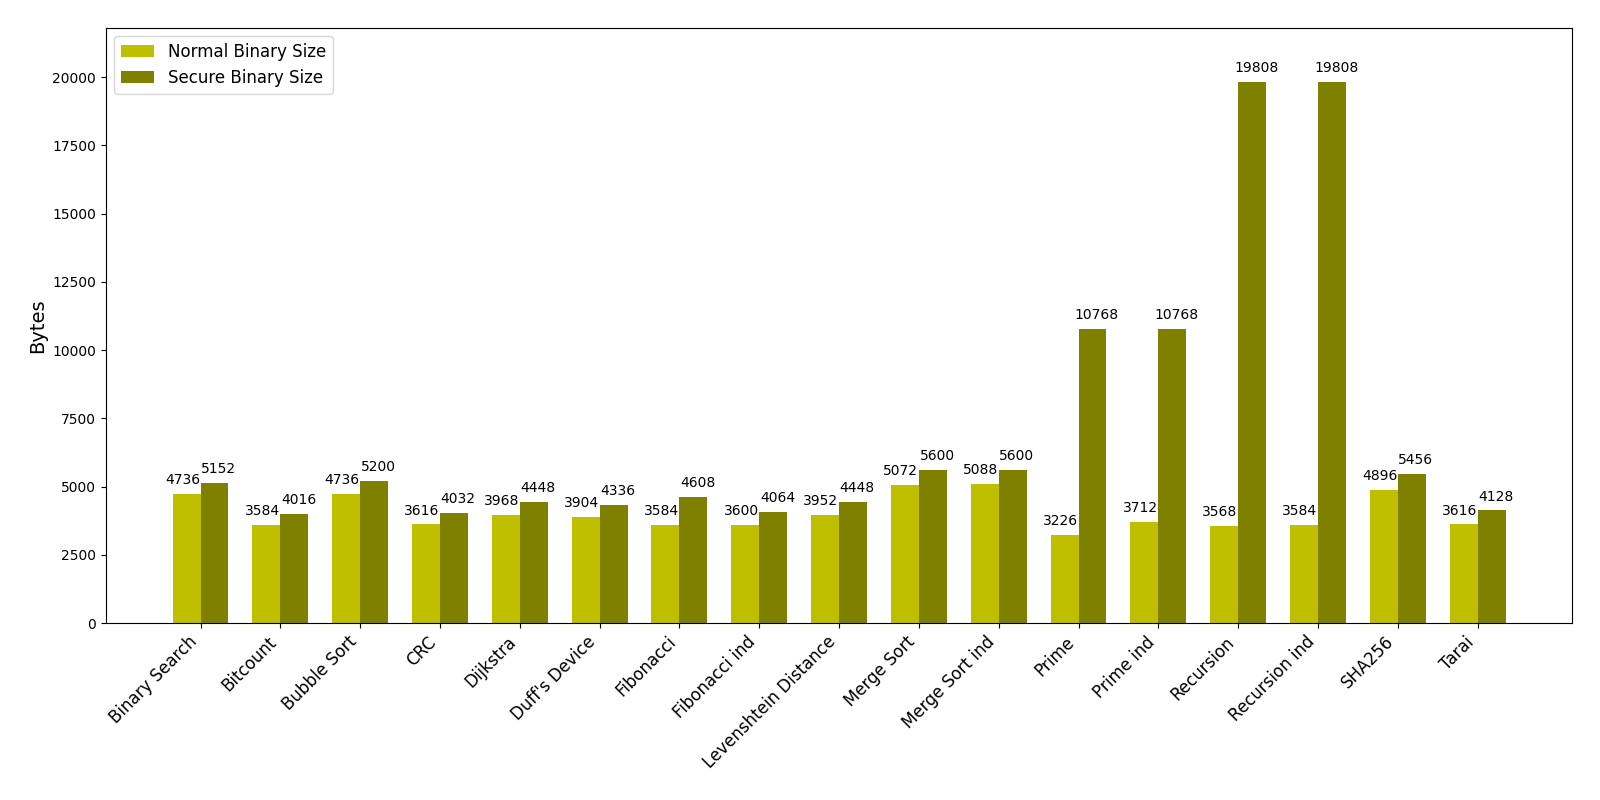
\includegraphics[width=.9\linewidth]{images/size.png}
  \caption{Comparison between binaries size}
  \label{fig:binsize}
\end{figure}

As we can see in Table \ref{tab:binsize}, in most cases the size of the binary
increases by $\sim 10\%$. This is due to the Shadow Stack, CFG, and the instructions
added during instrumentation.

As for the time analysis, there are some exceptions. \textit{Prime}, \textit{Recursion}
and their indirect variations present an overhead of $200\%$ or more. This happens
because these recursive algorithms perform all the jump instructions consecutively
and then all the return instructions. This means that we must allocate a Shadow
Stack big enough to store all the return addresses to ensure proper edge
controls. For example, we have seen that the \textit{Recursive} algorithm performs
$\sim 4000$ jump instructions, this means that we must create a Shadow Stack
that can store at least $4000$ addresses. Given that an address is stored as an \textit{unsigned
int}, we can easily see that a Shadow Stack that can store $4000$ addresses occupies
$4000*4 = 16000 \ \textit{Bytes}$\footnote{We multiply by $4$ because it is the
size of an \textit{unsigned int}.}. Now, if we take the size of the secure
binary for the \textit{Recursive} algorithm we can calculate $19808 - 16000 = 380
8 \ \textit{Bytes}$, so we can see that apart from the Shadow Stack the binary
has an overhead similar to the other ones.

Note that this problem is related strictly to recursive algorithms as they
perform a high number of jumps and then they start performing the first return
instruction. However, we could have a similar problem with the Control Flow
Graph as for a big binary like a firmware we can have many different jump
instructions and, as a consequence, the CFG would increase in size.

\begin{table}
  \centering
  \begin{tabular}{|c|c|c|c|}
    \hline
    \textbf{Algorithm}          & \textbf{Normal bin size (B)} & \textbf{Secure bin size (B)} & \textbf{Memory Overhead} \\
    \hhline{====} Binary Search & 4736                         & 5152                         & $8.78\%$                 \\
    \hline
    Bitcount                    & 3584                         & 4016                         & $12.05\%$                \\
    \hline
    Bubble Sort                 & 4736                         & 5200                         & $9.79\%$                 \\
    \hline
    CRC                         & 3616                         & 4032                         & $11.51\%$                \\
    \hline
    Dijkstra                    & 3968                         & 4448                         & $12.09\%$                \\
    \hline
    Duff's Device               & 3904                         & 4336                         & $11.06\%$                \\
    \hline
    Fibonacci                   & 3584                         & 4608                         & $28.57\%$                \\
    \hline
    Fibonacci Indirect          & 3600                         & 4064                         & $12.88\%$                \\
    \hline
    Levenshtein Distance        & 3952                         & 4448                         & $12.55\%$                \\
    \hline
    Merge Sort                  & 5072                         & 5600                         & $10.41\%$                \\
    \hline
    Merge Sort Indirect         & 5088                         & 5600                         & $10.06\%$                \\
    \hline
    Prime                       & 3226                         & 10768                        & $233.78\%$               \\
    \hline
    Prime Indirect              & 3712                         & 10768                        & $190.08\%$               \\
    \hline
    Recursion                   & 3568                         & 19808                        & $455.15\%$               \\
    \hline
    Recursion Indirect          & 3584                         & 19808                        & $452.68\%$               \\
    \hline
    SHA256                      & 4896                         & 5456                         & $11.43\%$                \\
    \hline
    Tarai                       & 3616                         & 4128                         & $14.16\%$                \\
    \hline
  \end{tabular}
  \caption{Test results for memory consumption}
  \label{tab:binsize}
\end{table}

Overall, \textit{project name} achieved an average memory overhead of $88.06\%$ with
a standard deviation of $152.77$. However, similarly to the space overhead, if
we do not take into consideration the outliers we can see that the median is
$1 2.09\%$. These results show that in most cases \textit{project name} can
produce a secure binary without affecting too much memory consumption. Even in this
case, the project suffers from recursive algorithms as we need to allocate a
bigger Shadow Stack to securely store each address.

\section{Results and Analysis}
\label{sec:pa_results}

In this section, we discuss the obtained result and showcase the weak point of
\textit{project name}.

As we have seen in the previous sections the project showcases promising performances
in most cases. In almost all the tested algorithms time overhead was barely
noticeable and memory consumption was acceptable. Overall, the project
infrastructure is not impacting the normal performances of the non-secure binary.

However, in the case of deeply recursive algorithms, we have seen that the time
overhead grows exponentially due to the high number of control transfer
instructions. Also, the size of the binary grows as we need a bigger Shadow
Stack to store all the addresses needed to perform the edge controls.

Moreover, we have seen that if the code is composed of thousands of lines it is likely
that the Control Flow Graph will be very big. This is because if we have many
jump instructions from different sources to different destinations we must store
each pair, thus the space occupied by the CFG grows.

In the following section, we provide some optimization techniques that could be
applied to further increase \textit{project name}'s performances. Specifically, we
provide alternative solutions to improve the weak points of the project.

\section{Optimization Techniques}
\label{sec:pa_optimization}

Since optimization is a key factor when developing projects on embedded devices
given their hardware limitations we tried to provide an infrastructure as fast
as possible while preserving memory usage. However, as test results show, there are
some aspects of the project that require further improvement to be considered acceptable.

The two identified edge cases from which the project suffers are:
\begin{itemize}
  \item Deeply recursive algorithms: we have seen that deeply recursive
    algorithms require a big Shadow Stack to hold all the return addresses and
    thus, they require a lot of memory. To solve this issue we could modify the
    Shadow Stack in the following way. When we see that a function calls itself many
    times we could store the return address only one time and introduce a \textit{peek}
    function. With this, we could still perform the backward edge controls when
    we need to but we would need to store the address only once. Then, if we
    need to perform a control on another address we would just need to \textit{pop}
    the ``recursive'' address and then \textit{pop} the following one to see if
    it matches with the one we are checking. With such modification, we could
    effectively reduce the amount of space occupied by the Shadow Stack without
    impacting the security features that the project provides;

  \item Big user code: we have seen that with very big codes (like the aforementioned
    firmware one) we could end up in a situation where the Control Flow Graph
    grows bigger and bigger due to the high amount of control transfer
    instructions from different sources to different destinations. Unfortunately,
    we can do nothing about memory consumption in this case as we can't afford
    to avoid storing some source-destination pairs. However, as already
    explained we could implement a Hash Table which would not decrease the
    memory consumption but, at least we could reduce the time required to access
    the Control Flow Graph from $\mathcal{O}(\log{n})$ to $\mathcal{O}(1)$.
\end{itemize}

Lastly, we provide a space optimization solution that could be implemented for
very small source codes. Say, for example, that the \textit{.text} section that
we want to instrument starts at address $0x4038a000$ and ends at address
$0x4038f000$. Since the first part of the address stays the same it provides no useful
information, thus we could apply a bit-mask to remove $4038$ from the address, storing
only the last $16$ bits. This means that we would be able to store an address
inside an \textit{unsigned short} instead of an \textit{unsigned int}. As a result,
we would be able to halve the space required to store the Control Flow Graph and
the Shadow Stack resulting in a great improvement in memory consumption. However,
this solution only works when the user code is very small because if the \textit{.text}
section starts at address $0x4038a000$ and ends at address $0x4050a000$ we would
still need an \textit{unsigned int} to store a correct representation of the
address.

In conclusion, we have seen that \textit{project name} offers good performances
but it has some edge cases where it impacts the performances severely. However,
it could be fine-tuned with the proposed solutions to adapt to specific
situations.
